\section{Interpretation et analyse des resultats}

% Les reponses a la question posee en introduction.

\subsection{Diagramme fondamental de reference}

% Campagne E0 : goulot sec seul.

\subsection{Effet de l'extraction repartie}

% Campagne E1.

\subsection{Premier banc : effet séparé des paramètres du sol mouillé}
\label{sec:mouille-un-parametre}

Avant les campagnes, le banc de couloir permet de séparer les mécanismes par
lesquels le sol mouillé agit. Le démonstrateur change à la fois la vitesse
souhaitée $s$, le temps de relaxation $\tau$ et l'accélération maximale
$a_{\max}$ de la bande mouillée ($4\leq x<\SI{8}{\metre}$), ce qui interdit
d'attribuer un effet à l'un d'eux. On part donc d'une référence où le mouillé
est identique au sec ($\tau=\SI{0.3}{\second}$,
$a_{\max}=\SI{3}{\metre\per\second\squared}$, $s=\SI{1.5}{\metre\per\second}$),
puis on reprend \emph{un seul} paramètre du mouillé à la fois
($\tau=\SI{0.6}{\second}$, $a_{\max}=\SI{0.7}{\metre\per\second\squared}$,
$s=\SI{1}{\metre\per\second}$), enfin des combinaisons. Les 24 agents, leurs
placements et les cinq graines sont les mêmes pour toutes les variantes ; les
écarts au passage médian sont appariés graine par graine. Ces valeurs restent
illustratives : il s'agit de séparer des mécanismes, pas de calibrer la piscine.

\begin{table}[ht]
\centering
\caption{Sol mouillé, un paramètre à la fois. Moyennes sur cinq graines ;
l'écart-type, de l'ordre de \SI{0.003}{\second} sur les temps, est omis.
Freinage : distance parcourue dans la bande avant de revenir à
\SI{5}{\centi\metre\per\second} de la vitesse souhaitée. Contacts : durée
cumulée des paires à moins de \SI{1}{\milli\metre} du contact dans la bande.}
\label{tab:mouille}
\begin{tabular}{lrrrr}
\toprule
Variante & $t_{50}$ (s) & Traversée (s) & Freinage (m) & Contacts (paires$\cdot$s) \\
\midrule
Référence (mouillé = sec) & 7,082 & 2,672 & 0,01 & 0 \\
Relaxation seule & 7,083 & 2,677 & 0,01 & 0 \\
Adhérence seule & 7,082 & 2,672 & 0,01 & 0 \\
Vitesse seule & 8,368 & 3,860 & 0,53 & 65 \\
Vitesse + adhérence & 8,324 & 3,816 & 0,73 & 63 \\
Complet (démonstrateur) & 8,223 & 3,716 & 1,86 & 55 \\
\bottomrule
\end{tabular}
\end{table}

\begin{figure}[ht]
\centering
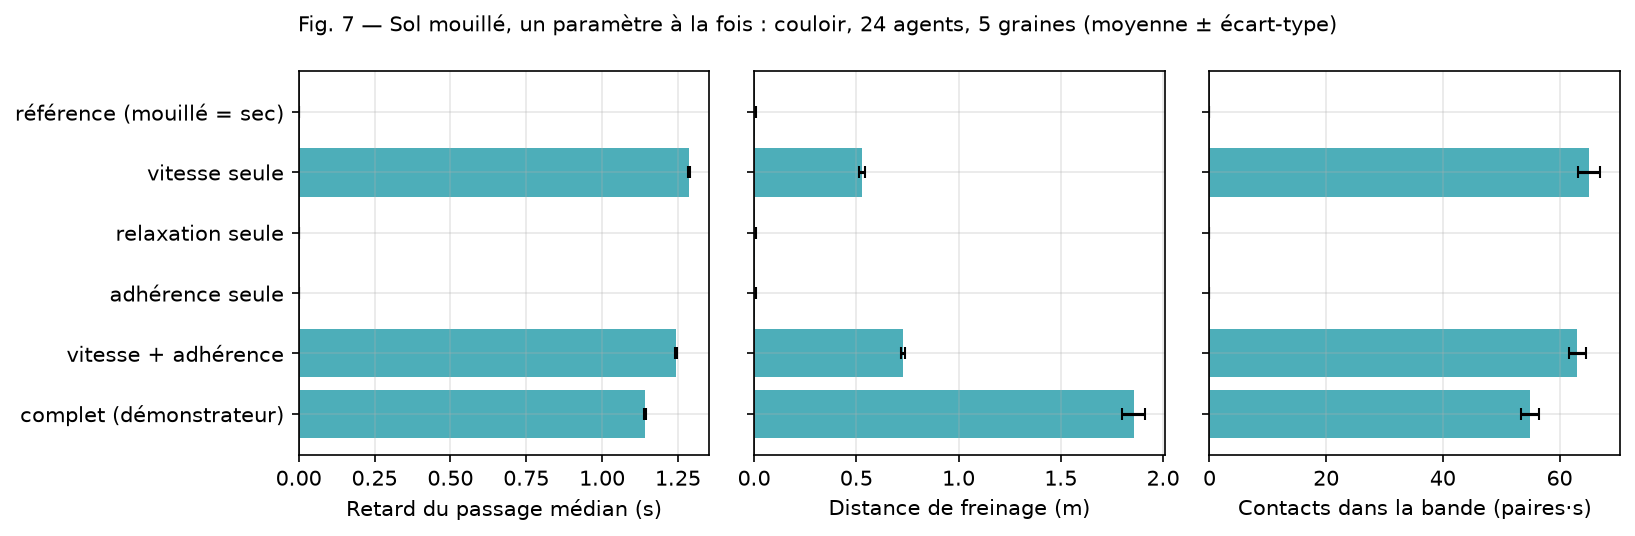
\includegraphics[width=\linewidth]{fig07_mouille_un_parametre}
\caption{Retard du passage médian par rapport à la référence, distance de
freinage et compression dans la bande mouillée, pour chaque variante.
Reproduction : \texttt{viscocrowd comparer-mouille experiments/couloir.yaml
--figure report/figures} (manifeste, figure 7).}
\label{fig:mouille}
\end{figure}

Trois constats se dégagent (tableau~\ref{tab:mouille} et
figure~\ref{fig:mouille}).

\paragraph{L'adhérence et la relaxation n'agissent que si la vitesse doit
changer.} À vitesse souhaitée identique, prendre seulement le $\tau$ ou
seulement le $a_{\max}$ du mouillé ne change rien : le passage médian bouge de
moins de \SI{1}{\milli\second} et aucun contact n'apparaît. Dans ce couloir droit,
les agents arrivent déjà à leur vitesse souhaitée ; rien ne leur demande
d'accélérer, de freiner ou de tourner. L'effet d'inertie étudié par la
problématique ne peut donc se manifester qu'à travers un \emph{transitoire} :
changement de vitesse souhaitée, virage, contournement ou collision.

\paragraph{La vitesse souhaitée retarde et comprime.} Seule, la vitesse plus
faible du mouillé retarde le passage médian de \SI{1.29}{\second}, un peu moins
que les \SI{1.33}{\second} d'une traversée à vitesse établie, puisque les agents
entrent dans la bande plus vite qu'ils ne la traversent. Les agents de tête
ralentissent avant ceux qui les suivent : la file se comprime à l'entrée, et
65~paires$\cdot$s de contacts apparaissent, contre aucun dans la référence.

\paragraph{Dans ce couloir, l'inertie allonge le freinage et réduit la
compression.} Avec une adhérence faible, le freinage demandé
($(1{,}5-1)/0{,}3\approx\SI{1.7}{\metre\per\second\squared}$) dépasse
$a_{\max}=\SI{0.7}{\metre\per\second\squared}$ et se trouve borné : la distance
de freinage passe de 0,53 à \SI{0.73}{\metre}, puis à \SI{1.86}{\metre} quand la
relaxation du mouillé s'ajoute. Les agents ralentissent alors plus
progressivement, la compression diminue (63 puis 55~paires$\cdot$s) et la bande est
traversée plus vite. C'est l'inverse de l'intuition « inertielle » de la
problématique, mais ce banc n'a ni virage ni goulot : l'inertie y étale le
ralentissement au lieu de provoquer des chocs. Le contournement d'un obstacle et
l'approche du goulot, où il faut tourner ou s'arrêter, restent les situations
qui départageront les hypothèses tampon et inertielle.

\subsection{Effet de l'inertie du carrelage mouille}

% Campagne E2, puis balayage E3. C'est le coeur du resultat : effet tampon ou
% effet inertiel, et de quelle amplitude.

\subsection{Sensibilite aux parametres de scenario}

% Campagne E4.
